The simulation workflow~\ref{fig:fluxo_simulacao} employs three tools: the QuaDRiGa channel generator, a Python simulator developed in this work, and C++ code developed in Vitis HLS, which computes the inverse of $\mathbf{G}_c$ using fixed-point arithmetic. QuaDRiGa generates the channel matrices $\mathbf{H}$ for the target UEs and $\overline{\mathbf{H}}$ for the interfering UEs.

The Python simulator handles the transmission process. It generates symbols for the target UEs and creates colored noise, with a covariance derived from $\overline{\mathbf{H}}$ (Section~\ref{subsec:ruido-colorido}), to construct the received signal using $\mathbf{H}$. Subsequently, it computes the equalizers, performs symbol detection, and measures the SER at various SNR levels. The BCD-MMSE algorithm is simulated in two ways: using the inverse of $\mathbf{G}_c$ in 64-bit floating-point format (which serves as a reference) and using the inverse in fixed-point format. In the latter case, whenever the BCD-MMSE algorithm requires $\mathbf{G}_c^{-1}$, the Python simulator invokes the C++ code.

The Python simulator models the same uplink as in \cite{zhao2025jsac}. According to the authors, that paper was the first work on decentralized processing to consider colored noise \cite{zhao2025jsac}. Therefore, the simulation parameters follow that work, except where the text indicates otherwise.



% Fluxo conferido no código:
%   QuaDRiGa: software/simulador/quadriga/export_quadriga_channels.m (semente: linha 83)
%   laço e equalizadores: dbp_sim/m1_driver.py:149-211; dbp_sim/m7_equalizers.py
%     (lmmse, zero_forcing, bdac_mmse, bcd_mmse_path); Ledoit-Wolf: dbp_sim/m5_noise.py:162-168
%   inversa em ponto fixo: dbp_sim/hls_inverse.py (usada nos resultados de SER,
%     varredura_formatos.py, bcd_inverse="hls") e dbp_sim/hw_inverse.py (modelo em Python)
% Conteúdo vem de constraints/diagramas/fluxo_simulador.puml; estrutura em caixas do
% rascunho constraints/diagramas/metodologia.svg.
\begin{figure}[!ht]
\caption{Simulation flow: QuaDRiGa channels, Python simulator and fixed-point inverse.}
\label{fig:fluxo_simulacao}
\vspace{4pt} % a classe zera o espaço entre a caption e a figura
\centering
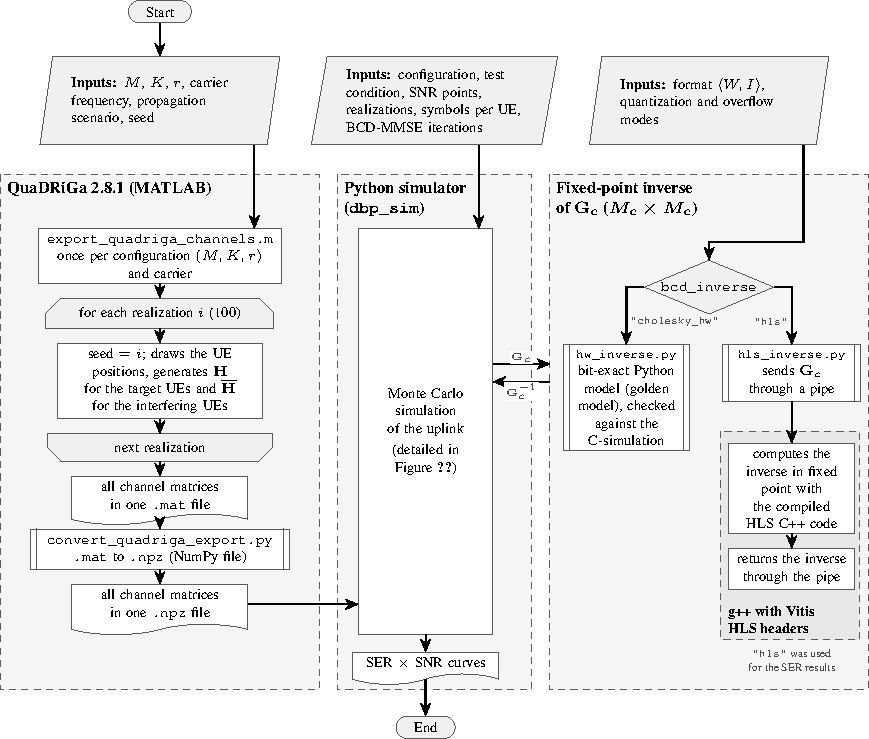
\includegraphics{Images/FLUXO/simulacao_a.pdf}
\vspace{4pt}
\legend{Source: the author.}
\end{figure}

% ---------------------------------------------------------------------
\subsection{\texorpdfstring{Channel generation}{Channel generation}}\label{subsec:simul-canal}
% ---------------------------------------------------------------------
The channels are generated using QuaDRiGa 2.8.1 in MATLAB. They depend on the number of antennas $M$, the number of target UEs $K$, the number of interfering UEs $r$, and the carrier frequency. Consequently, they are generated once for each combination of these values. Other parameters, such as $C$, the modulation scheme, and the IoTh, only affect the processing steps within the Python-based simulator. The simulation employs 100 channel realizations. Each realization consists of a random selection of UE positions, along with the corresponding channels $\mathbf{H}$ and $\overline{\mathbf{H}}$ generated by QuaDRiGa for those specific positions. Every realization uses its own unique random seed.


MATLAB saves the channels for all 100 realizations into a \texttt{.mat} file. A Python script then converts this file into an \texttt{.npz} file, NumPy’s format for storing multiple arrays within a single compressed file. The Python-based simulator reads the matrices $\mathbf{H}$ and $\overline{\mathbf{H}}$ from this file.
% ---------------------------------------------------------------------
\subsection{\texorpdfstring{Python simulator}{Python simulator}}\label{subsubsec:simul-python}
% ---------------------------------------------------------------------
The Python simulator runs two nested loops (Figure~\ref{fig:fluxo_python}). The outer loop iterates through the 100 realizations, while the inner loop iterates through the SNR points. The SNR points range from $-10$ to $10$~dB, with a step of $2$~dB. For each realization, the simulator takes $\mathbf{H}$ and $\overline{\mathbf{H}}$ corresponding to that realization and uses these channels across all SNR points. Each point on the SER curves represents the average over the 100 realizations. This is a Monte Carlo simulation, as in \cite{zhuang2025}: the SER (Section~\ref{subsubsec:ser}) is estimated by the fraction of erroneous symbols across many random draws of the channel, noise, and symbols.

At each SNR point, the simulator constructs the noise covariance matrix based on $\overline{\mathbf{H}}$, the IoTh (interference-over-thermal), and the SNR. It then generates $N$ noise samples, $\mathbf{n}^i$ (Section~\ref{subsubsec:estimacao-R}). It also generates 480 data symbols for each UE, along with the noise associated with these symbols. Based on this, the equalizers are calculated. The channel remains constant within the coherence block (Section~\ref{subsec:bloco-coerencia}); therefore, each equalizer is computed once and applied to all 480 symbols. The BCD-MMSE is compared against two centralized equalizers, the LMMSE and the ZF, which serve as benchmarks. The ZF does not utilize the noise samples $\mathbf{n}^i$. In contrast, both the LMMSE and the BCD-MMSE employ these samples to estimate the noise covariance (Section~\ref{subsubsec:condicionamento-R}). This estimate is always subjected to Ledoit-Wolf shrinkage (Equation~\ref{eq:ledoit-wolf}) before being used, even in cases where the estimate is already invertible.

In the LMMSE, this adjustment is applied to the estimate $\hat{\mathbf{R}}$ corresponding to all $M$ antennas. In the BCD-MMSE, each DU performs the adjustment on its own block, $\hat{\mathbf{R}}_{cc}$, using only the samples from its $M_c$ antennas. Consequently, no DU requires access to the samples from any other DU. The adjusted block forms the matrix $\mathbf{G}_c$ (Section~\ref{subsec:bcd}). In the reference version of the BCD-MMSE, this matrix is inverted using 64-bit floating-point arithmetic; alternatively, it can be inverted using fixed-point arithmetic (Section~\ref{subsubsec:simul-inversa}).



\begin{figure}[!ht]
\caption{Detailed flow of the Python simulator: Monte Carlo loop, equalizers and SER.}
\label{fig:fluxo_python}
\vspace{4pt} % a classe zera o espaço entre a caption e a figura
\centering
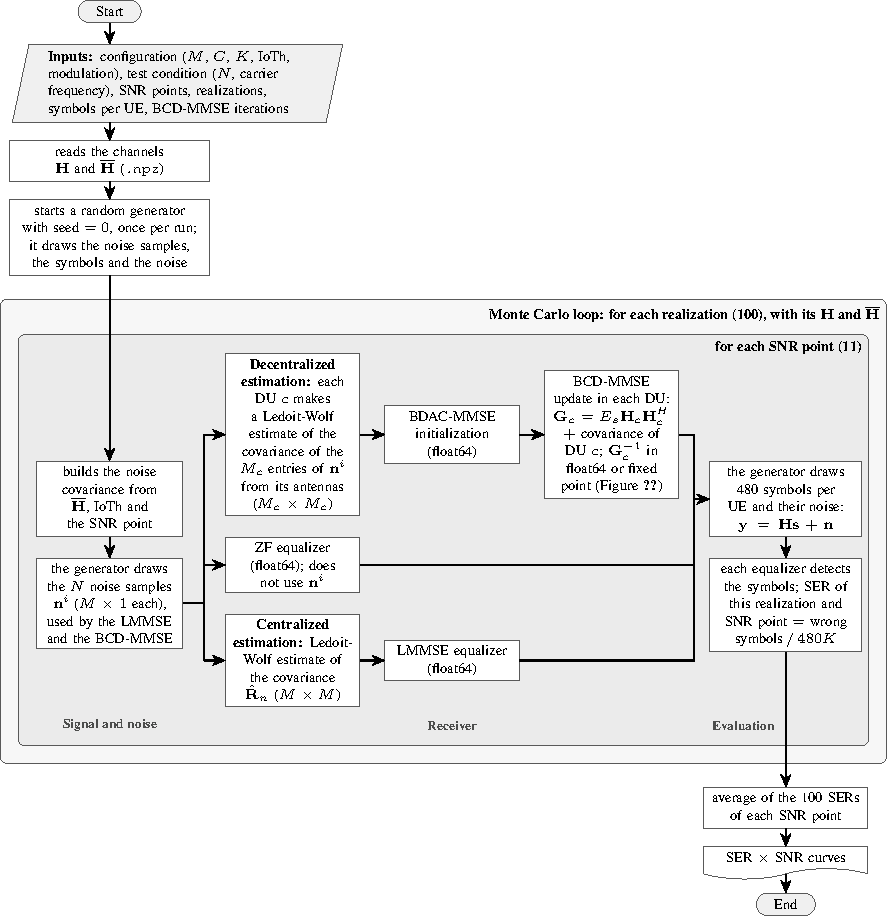
\includegraphics{Images/FLUXO/simulacao_b.pdf}
\vspace{4pt}
\legend{Source: the author.}
\end{figure}

% ---------------------------------------------------------------------
\subsection{\texorpdfstring{Fixed-point inverse}{Fixed-point inverse}}\label{subsubsec:simul-inversa}
% ---------------------------------------------------------------------
The inverse of $\mathbf{G}_c$ in fixed-point arithmetic is derived from the C++ code of the inversion module (Section~\ref{subsec:hw-modulo}). This code is compiled using \texttt{g++} along with the \texttt{ap\_fixed} header files from Vitis HLS 2026.1, with a separate compilation performed for each combination of format $\langle W, I\rangle$, quantization mode, overflow mode (Table~\ref{tab:modos-apfixed}), and size $M_c$. The program remains active throughout the simulation. Other calculations within the simulator, including the inverses used for BDAC initialization and LMMSE, utilize 64-bit floating-point arithmetic.

To verify this program, the same $\mathbf{G}_c$ matrices used in the simulator were inverted both by this program and by the Vitis HLS C-simulation. This process involved 30 matrices for each of the 35 mode combinations, with $M_c$ set to 16 and 32. In every instance, the resulting inverses were bit-identical. Consequently, the Symbol Error Rate (SER) is measured using the exact same inverse as that calculated by the hardware. The simulator also includes a Python-based model of the inversion, which has been verified bit-for-bit against the C++ code; however, the reported SER results are based on the C++ implementation.

% REMOVIDO (2026-11-05): subseção "Flow diagram". A Figura fig:fluxo_simulacao foi para a
%   abertura da seção; a frase da subseção ficou redundante com a abertura.

